Needed to \textbf{avoid digestion of mRNA}
by nucleases (foreign body response) and to
facilitate endocytosis.\\

\begin{minipage}
    {0.3\linewidth}
    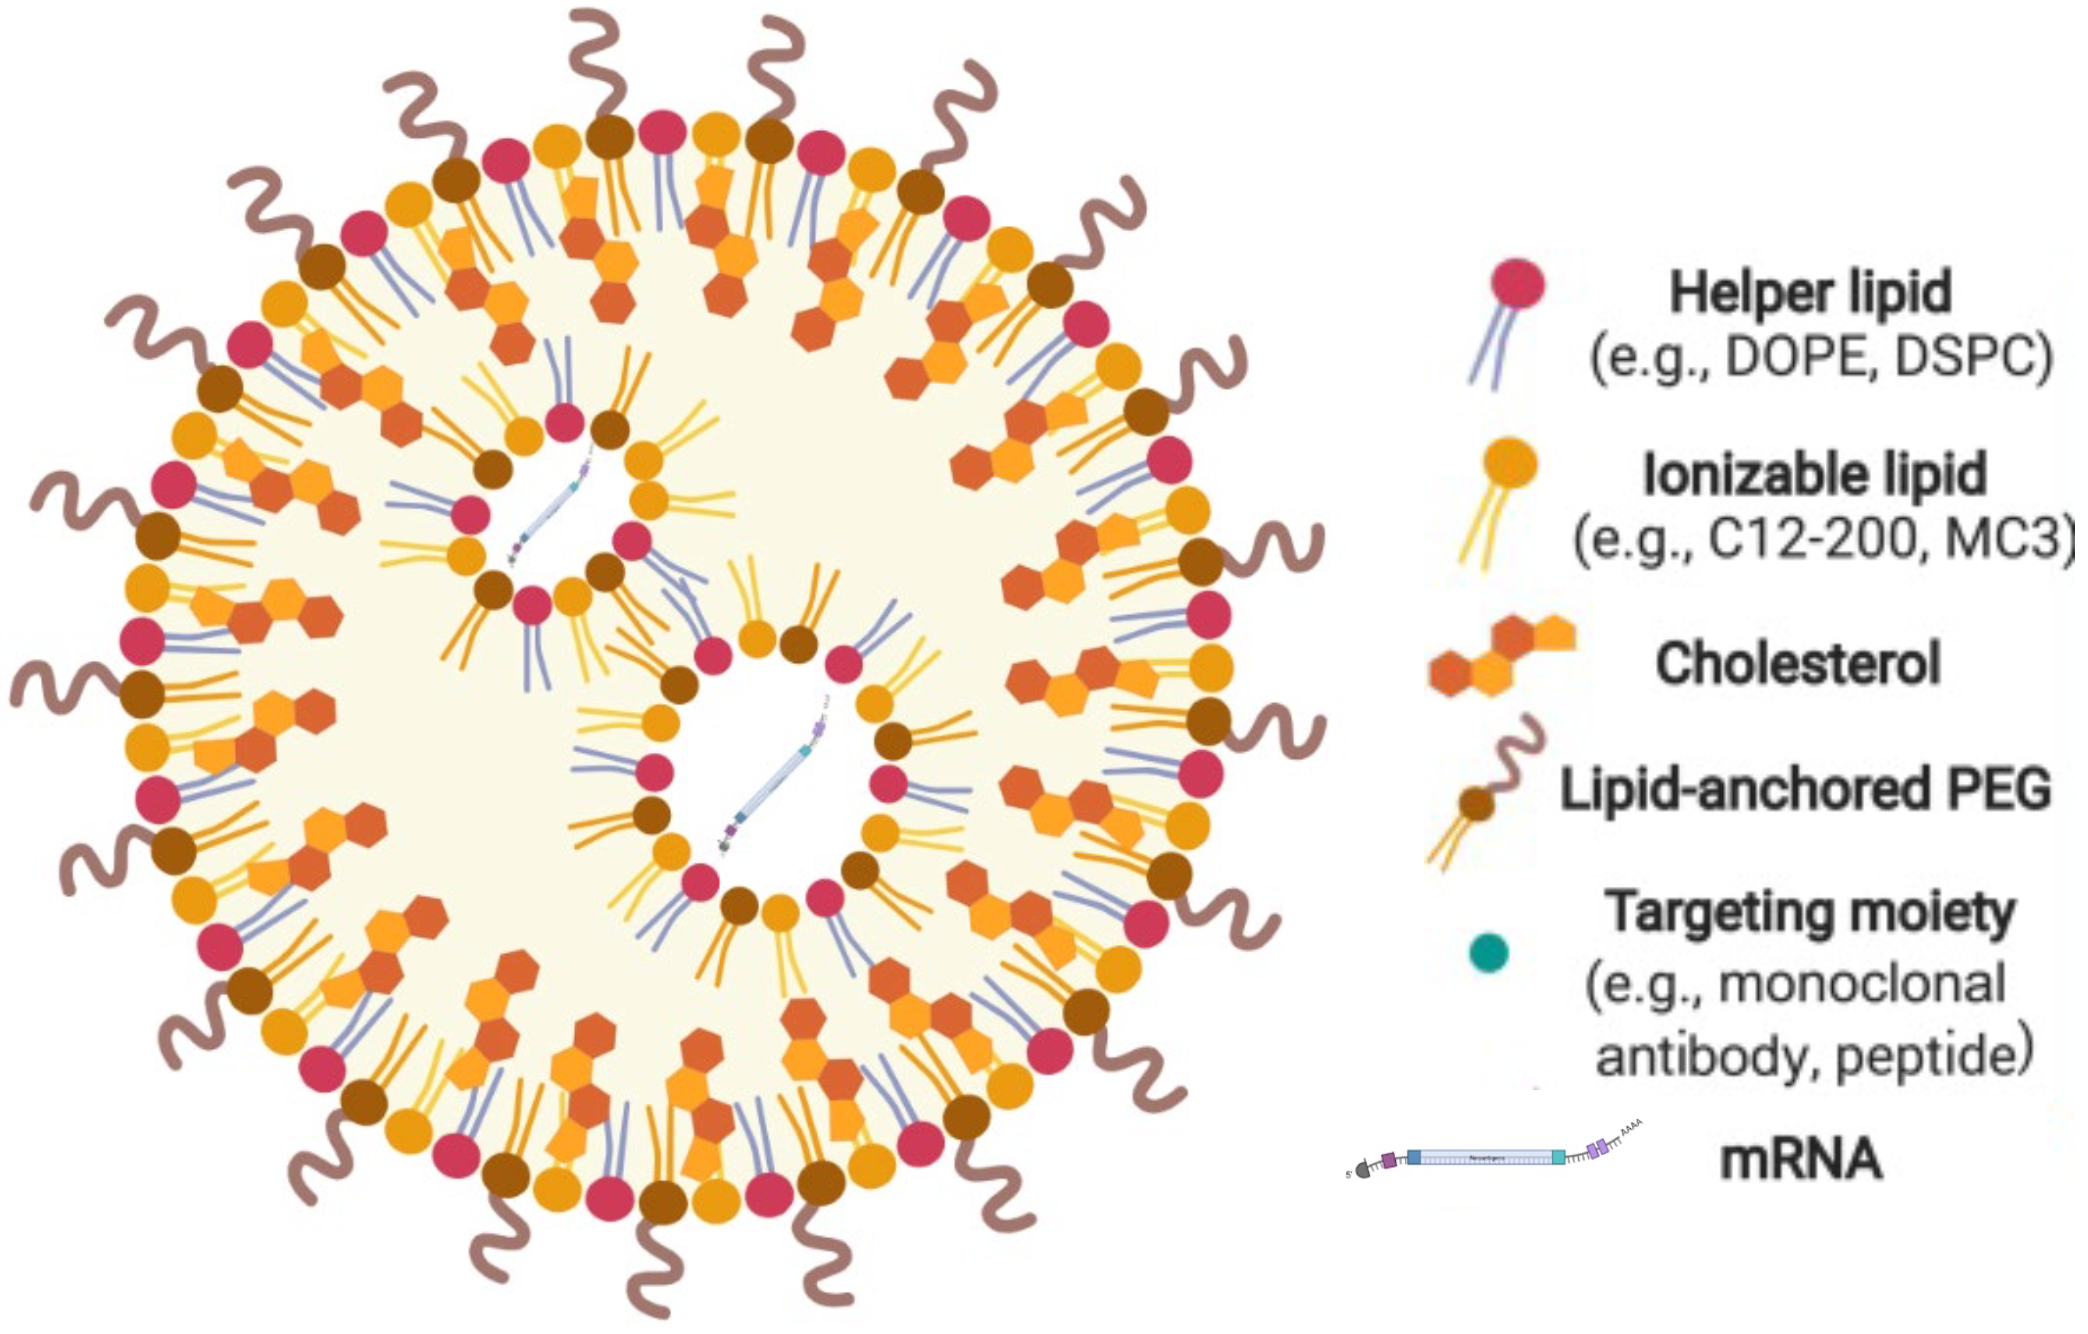
\includegraphics[width=25mm]{src/Images/lnp.png}
\end{minipage}
\begin{minipage}
    {0.7\linewidth}
LNP include 4 \textbf{main components}:
    \begin{itemize}
        \item \textbf{phospholipids:} stabilize shape
        \item \textbf{ionizable lipids:} help RNA to escape endosome
        \item \textbf{cholesterol:} reduce permeability
        \item \textbf{PEGylated lipids:} help avoid immune response
    \end{itemize}
\end{minipage}\\

How are \textbf{LNPs assembled}?
\begin{itemize}
    \item \textbf{Lipids and cholesterol} are dissolved in an \textbf{organic phase} (e.g. ethanol)
    \item \textbf{mRNA} is dissolved in an \textbf{aqueous buffer} (low pH)
    \item \textbf{Rapid mixing} of both phases leads to LNPs assembly
\end{itemize}